\documentclass[12pt,a4paper]{article}
\usepackage{geometry}
\geometry{left=2.5cm,right=2.5cm,top=2.0cm,bottom=2.5cm}
\usepackage{CJKutf8}
\usepackage[english]{babel}
\usepackage{amsmath,amsthm}
\usepackage{amsfonts}
\usepackage[longend,ruled,linesnumbered]{algorithm2e}
\usepackage{fancyhdr}
\usepackage{array}
\usepackage{listings}
\usepackage{color}
\usepackage{graphicx}
\graphicspath{ {./img/} }

\begin{document}
\begin{CJK*}{UTF8}{gbsn}

	\title{
		{\textbf《算法分析与设计》第 {$3$} 次作业
			\footnote{要求:1、分析题请用书面化语言给出详细分析过程。2、作业请统一使用hw0*-学号-姓名的命名格式,latex版本请附上源代码并打包提交。}
		}
	}
	\date{}

	\author{
		姓名:\underline{王骏}~~~~~~
		学号:\underline{71119138}~~~~~~
		成绩:\underline{~~~~~~~~~~~~~~~~~~}
	}

	\maketitle

	\noindent
	\section*{\bf \color{red}{算法分析题}}
	\noindent
	{\bf 题目1:}假设矩阵$A$、$B$、$C$、$D$、$E$的维数序列为$ <5,\ 10,\ 3,\ 12,\ 5,\ 50>$, 用动态规划算法找出其最佳连乘顺序。为方便起见,将矩阵连乘积 $A_iA_{i+1}...A_j$ 简记为 $A[i:j]$。
	\begin{enumerate}
		\item[(a)]  若将计算 $A[i:j]$ 所需的最少乘法次数记为 $m[i,j]$,请给出 $m[i,j]$ 的递推方程(即递归定义);
		\item[(b)]  若将对应于 $m[i,j]$ 的最佳断开位置记为 $s[i,j]$ 。根据上述实例,写出 $m[i:j]$ 表和 $s[i,j]$ 表的填充过程,并结合这两张表给出该实例的最佳连乘顺序。
	\end{enumerate}

	\vspace{5pt}
	\noindent
	{\bf 答:}

	(a)

	$$
	m[i,j]= \left\{\begin{array}{lcl}
			\min\limits_{i \leq k<j} \{m[i][k] + m[k+1][j] + p_{i-1}p_kp_j\} & \mbox{for} & i < j \\
			0 & \mbox{for} & i=j
		\end{array}\right
		$$

		(b)

		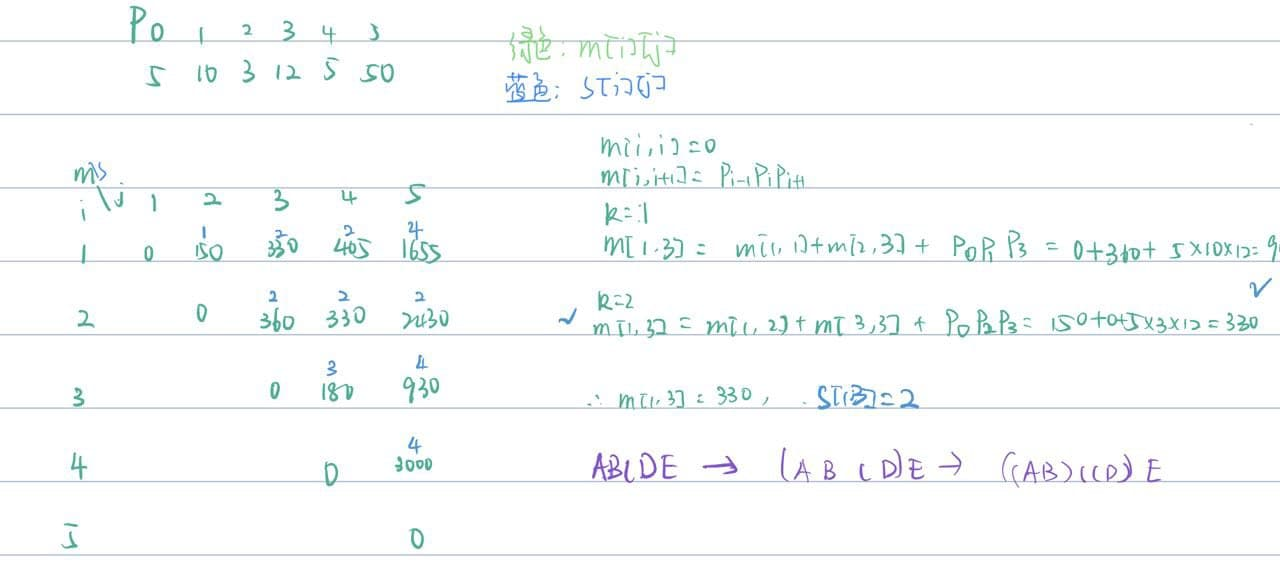
\includegraphics[width=15cm]{img/answ1.jpg}

		\vspace{10pt}
		\noindent
		{\bf 题目2:}假设我们要将一根大型长钢管锯成若干段。我们在要锯的地方打上标记,一共是 $n$ 个标记。这些标记距离钢管左端的距离,从左到右,分别是 $a_1,\ a_2,\  ...,\ a_n$ 厘米。这个钢管的总长是 $l$ 厘米,$l > a_n$ (参见下图)。当我们将钢管锯为两截时,需要的代价与当时被锯钢管的长度成正比,比例是每一厘米 $p$ 元。\\
		\begin{figure}[h]
			\centering %图片居中
			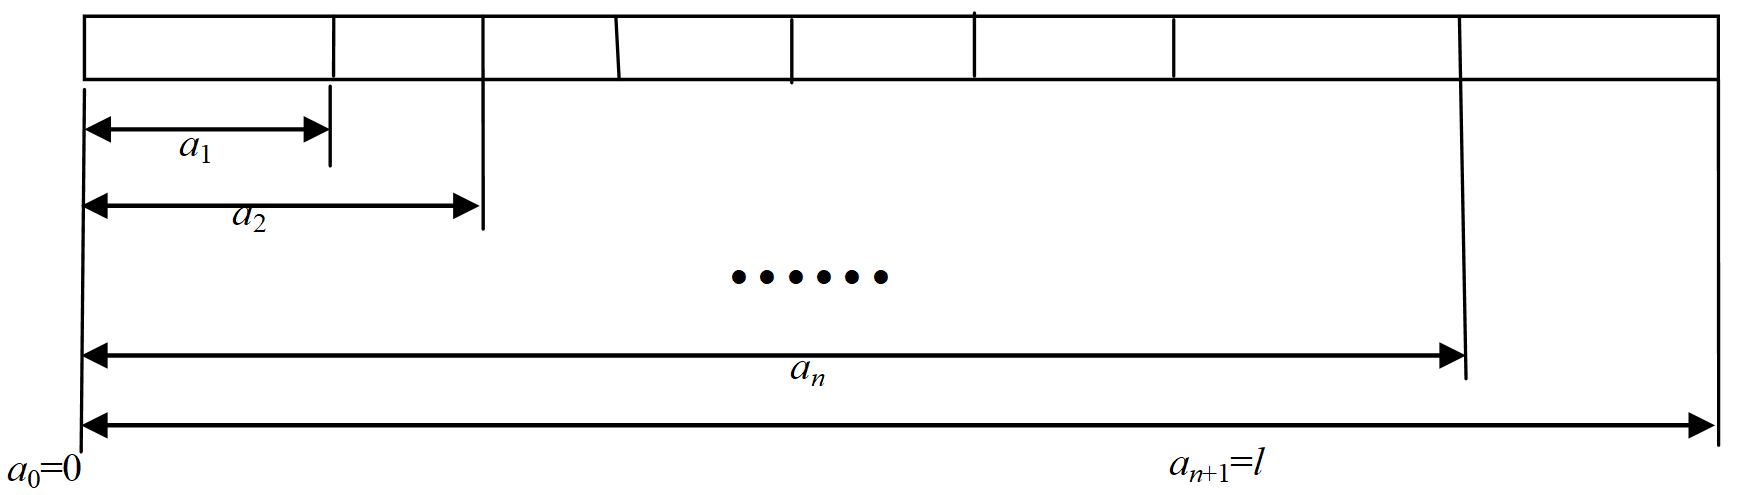
\includegraphics[width=0.7\textwidth]{2} %插入图片,[]中设置图片大小,{}中是图片文件名
		\end{figure}	

		\begin{enumerate}
			\item[(a)]  请用动态规划的方法设计一个算法来找出最优的顺序来完成这 $n$ 处的切割使总的代价最小。分析你的算法的复杂度。 (提示:用 $a_0 = 0$ 和 $a_{n+1} = l$ 表示钢管左端和右端位置。用$[a_i, a_j]$表示从标记 $a_i$ 到 标记 $a_j$ 这段钢管。用 $C(i,\ j)$ 表示完成对 $[a_i,\ a_j]$ 这段钢管的切割任务所需的最小代价,也就是完成所有 $a_k (i < k < j)$ 处的切割所需代价。 找出 $C(i, j)$ 的归纳公式。)
			\item[(b)]  以下面数据为例,用你在(a)中的算法找出最优的切割顺序和总代价。请显示你的计算过程。\\
				$a_1 = 2, a_2 = 5, a_3 = 9, a_4 = 14, l = 15, p = 1$.
		\end{enumerate}

		\vspace{5pt}
		\noindent
		{\bf 答:}

		(a)
		\begin{itemize}
			\item Algorithm
				$$
				C[i,j]= \left\{\begin{array}{lcl}
						\min\limits_{i \leq k<j} \{C[i][k] + C[k][j] + p(a_j - a_i)\} & \mbox{for} & i < j + 1 \\
						0 & \mbox{for} & j=i+1
					\end{array}\right
					$$
				\item 算法步骤与矩阵连乘一样,斜向列表,并记录每个k到s[i][j], 再通过k逆向切割管子 
				\item 复杂度同矩阵连乘: \mathcal{O}(n^3) 

			\end{itemize} (b) 

			Flow:

			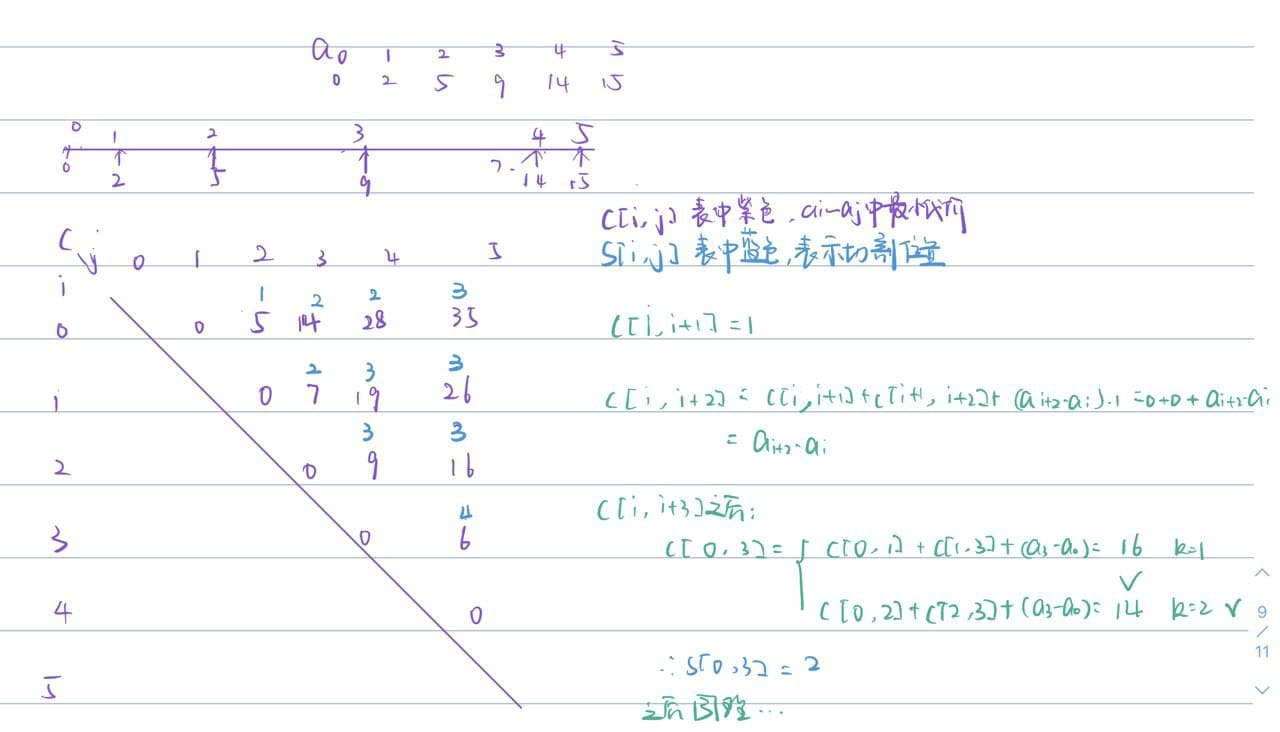
\includegraphics[width=15cm]{img/answ2.jpg}

			Result:

			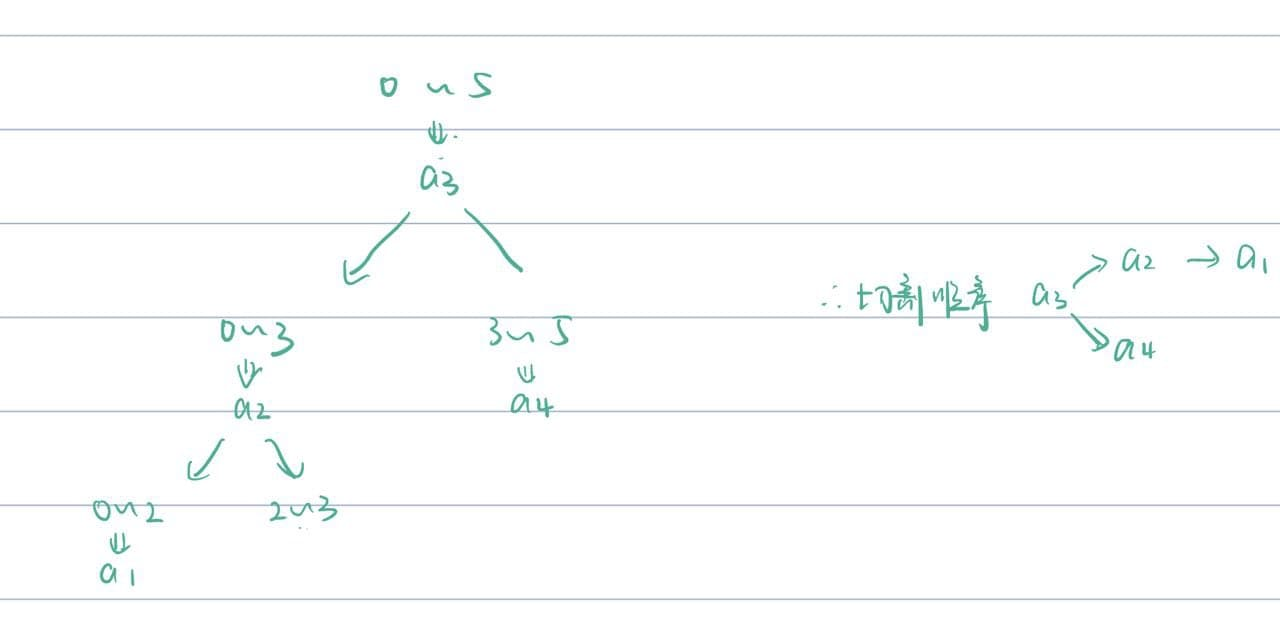
\includegraphics[width=15cm]{img/answ2_2.jpg}

			\vspace{10pt}
			\noindent
			{\bf 题目3:}假设我们有三个字母或数字的序列,$X[1..m]  = x_1x_2 ... x_m$, $Y[1..n]  = y_1y_2...y_n$,和 $Z[1..m+n] = z_1z_2...z_{m+n}$ 。如果序列 $Z$ 是由 $X$ 和 $Y$ 中的元素按顺序交汇而成,那么 $Z$  被称为 $X$ 和 $Y$ 的一个洗牌。例如,下面图中的序列 $Z = cchocohilaptes$ 是 $X = chocolate$ 和 $Y = chips$ 的一个洗牌 。
			\begin{figure}[h]
				\centering %图片居中
				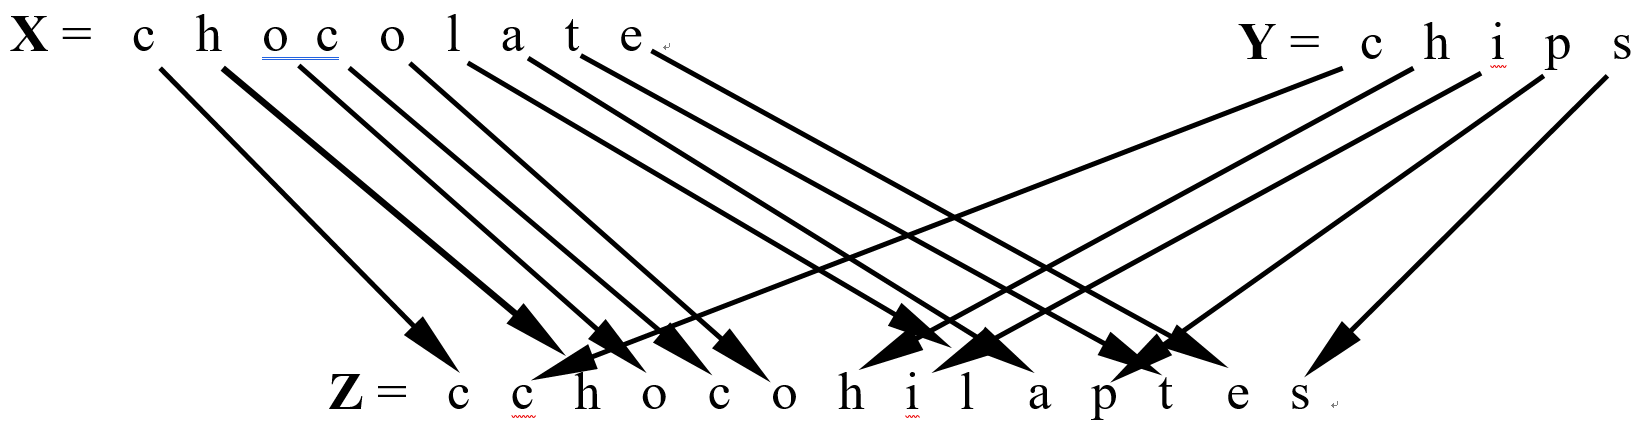
\includegraphics[width=0.7\textwidth]{3} %插入图片,[]中设置图片大小,{}中是图片文件名
			\end{figure}
			\begin{enumerate}
				\item[(a)]  用动态规划的方法设计一个算法来确定序列 $Z$ 是否是 $X$ 和 $Y$ 的一个洗牌。(提示:用 $M[i, j] = 1$ 表示 $Z[1..i+j]$ 是 $X[1..i]$ 和 $Y[1..j]$ 的一个洗牌。然后找出归纳公式。)
				\item[(b)]  用你的算法确定以下三序列中,$Z$ 是否是 $X$ 和 $Y$ 的一个洗牌。\\
					$X = FEAST, 	Y = LOVE, 	Z =  FLOEVASET$.
			\end{enumerate}
			\vspace{5pt}
			\noindent
			{\bf 答:}

			(a) Algorithm:

			\begin{itemize}
				\item 记M[i][j] = 1 表示 Z[1, i+j] 是X[i], Y[j] 的洗牌
				\item 递归公式 $$
					Z[i+j] = \left\{\begin{array}{lcl}
							X[i] & \Rightarrow & M[i-1][j] = 1\\
							Y[j] & \Rightarrow & M[i][j-1] = 1\\
							not Equal Either& \Rightarrow & M[i,j] = 0
						\end{array}
						$$
					\item M[0][0] = 0
				\end{itemize}

				(b) 

				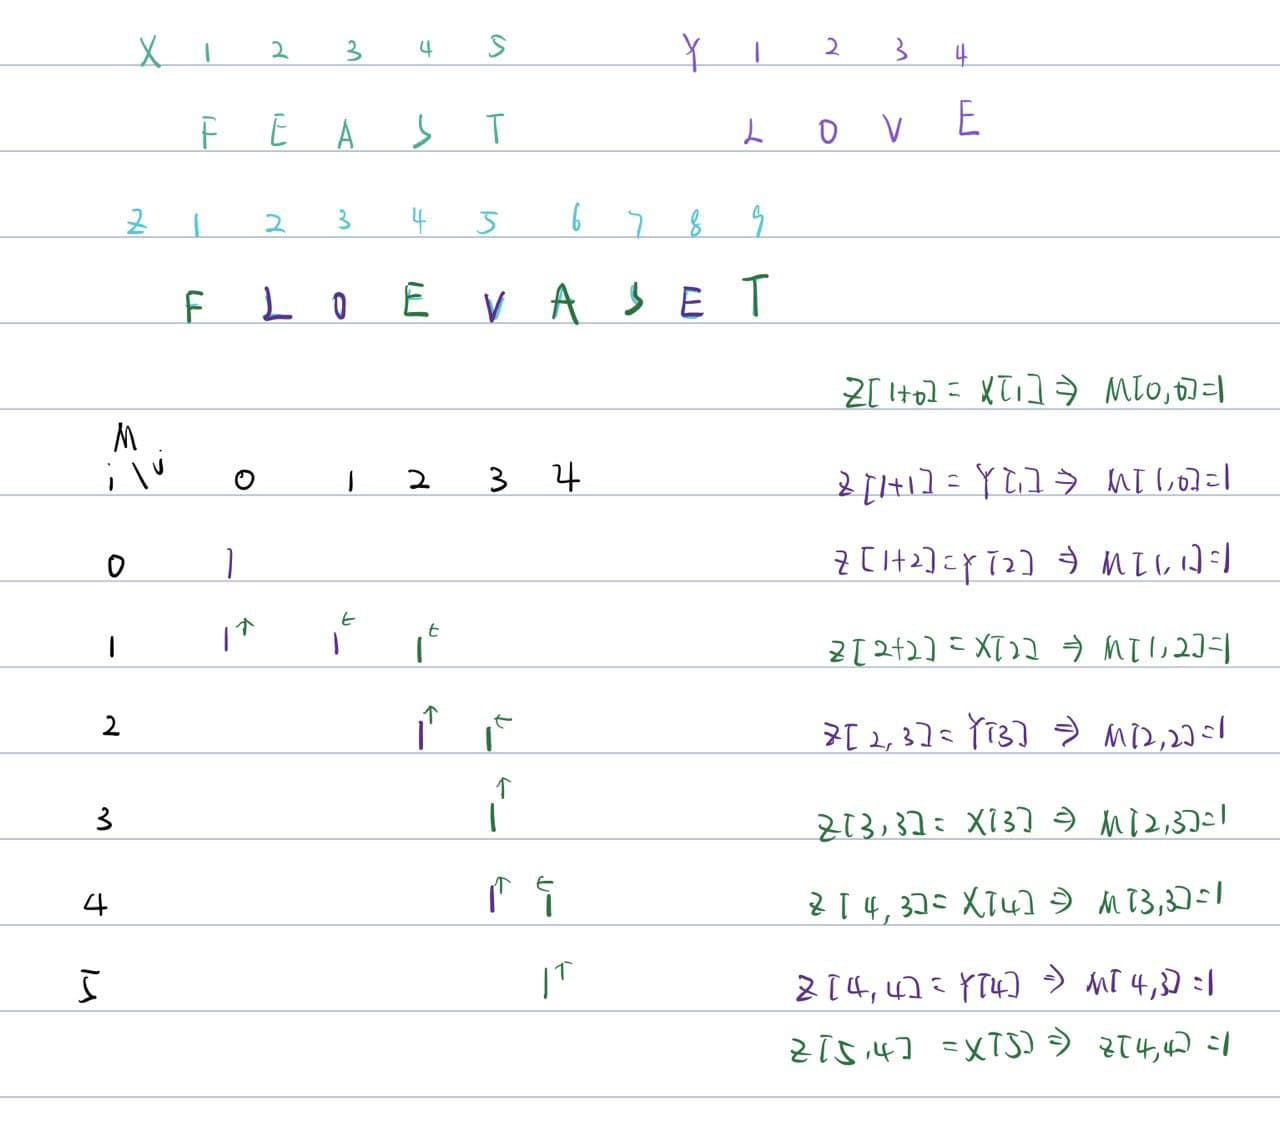
\includegraphics[width=15cm]{img/answ3.jpg}

				所以是一个洗牌
			\end{CJK*}
			\end{document} 
